\subsection{Sun Scan}
We performed sun scans with two different settings.
A step size of \SI{0.5}{\degree} with a total scan width of \SI{20}{\degree} and a step size of \SI{0.1}{\degree} with a total scan width of \SI{10}{\degree}.
For each of the settings we performed a horizontal and a vertical scan centered around the sun.
The integrated power spectra are then each normalized by subtracting the minimum and then dividing with the (new) maximum.
These normalized values are shown in figures \ref{fig:sun_scan}

\begin{figure}[ht]
    \centering
    \begin{subfigure}[t]{0.45\linewidth}
        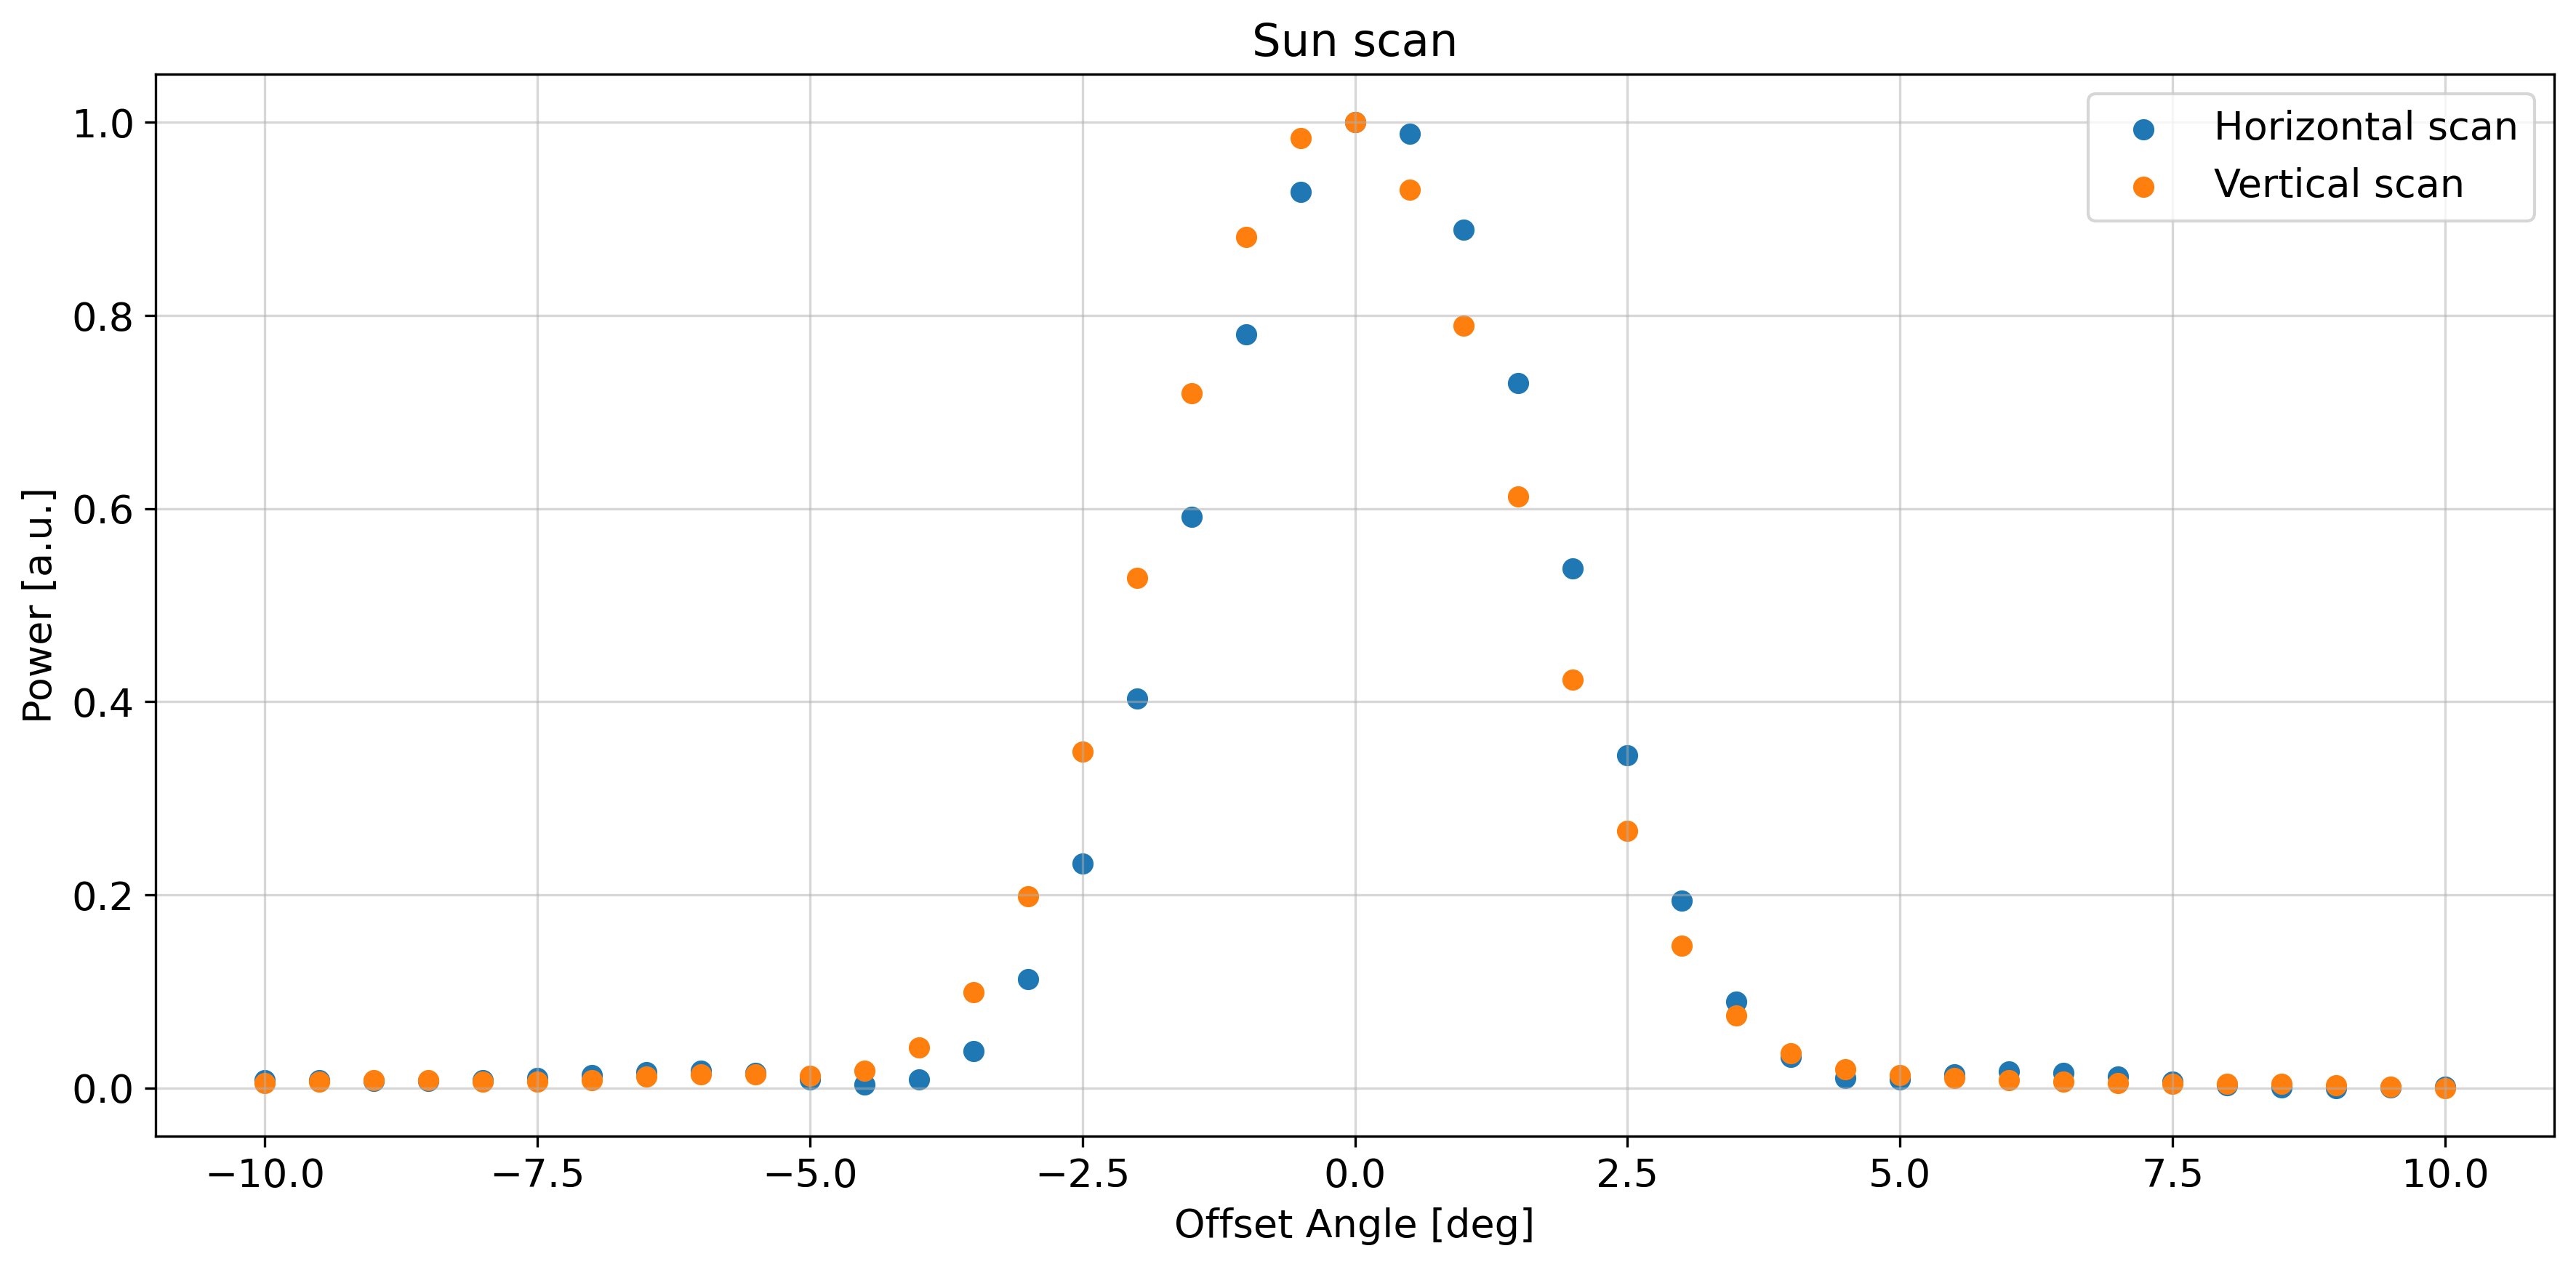
\includegraphics[width=\linewidth]{assets/sun_scan_low_res.png}
    \end{subfigure}
    \begin{subfigure}[t]{0.45\linewidth}
        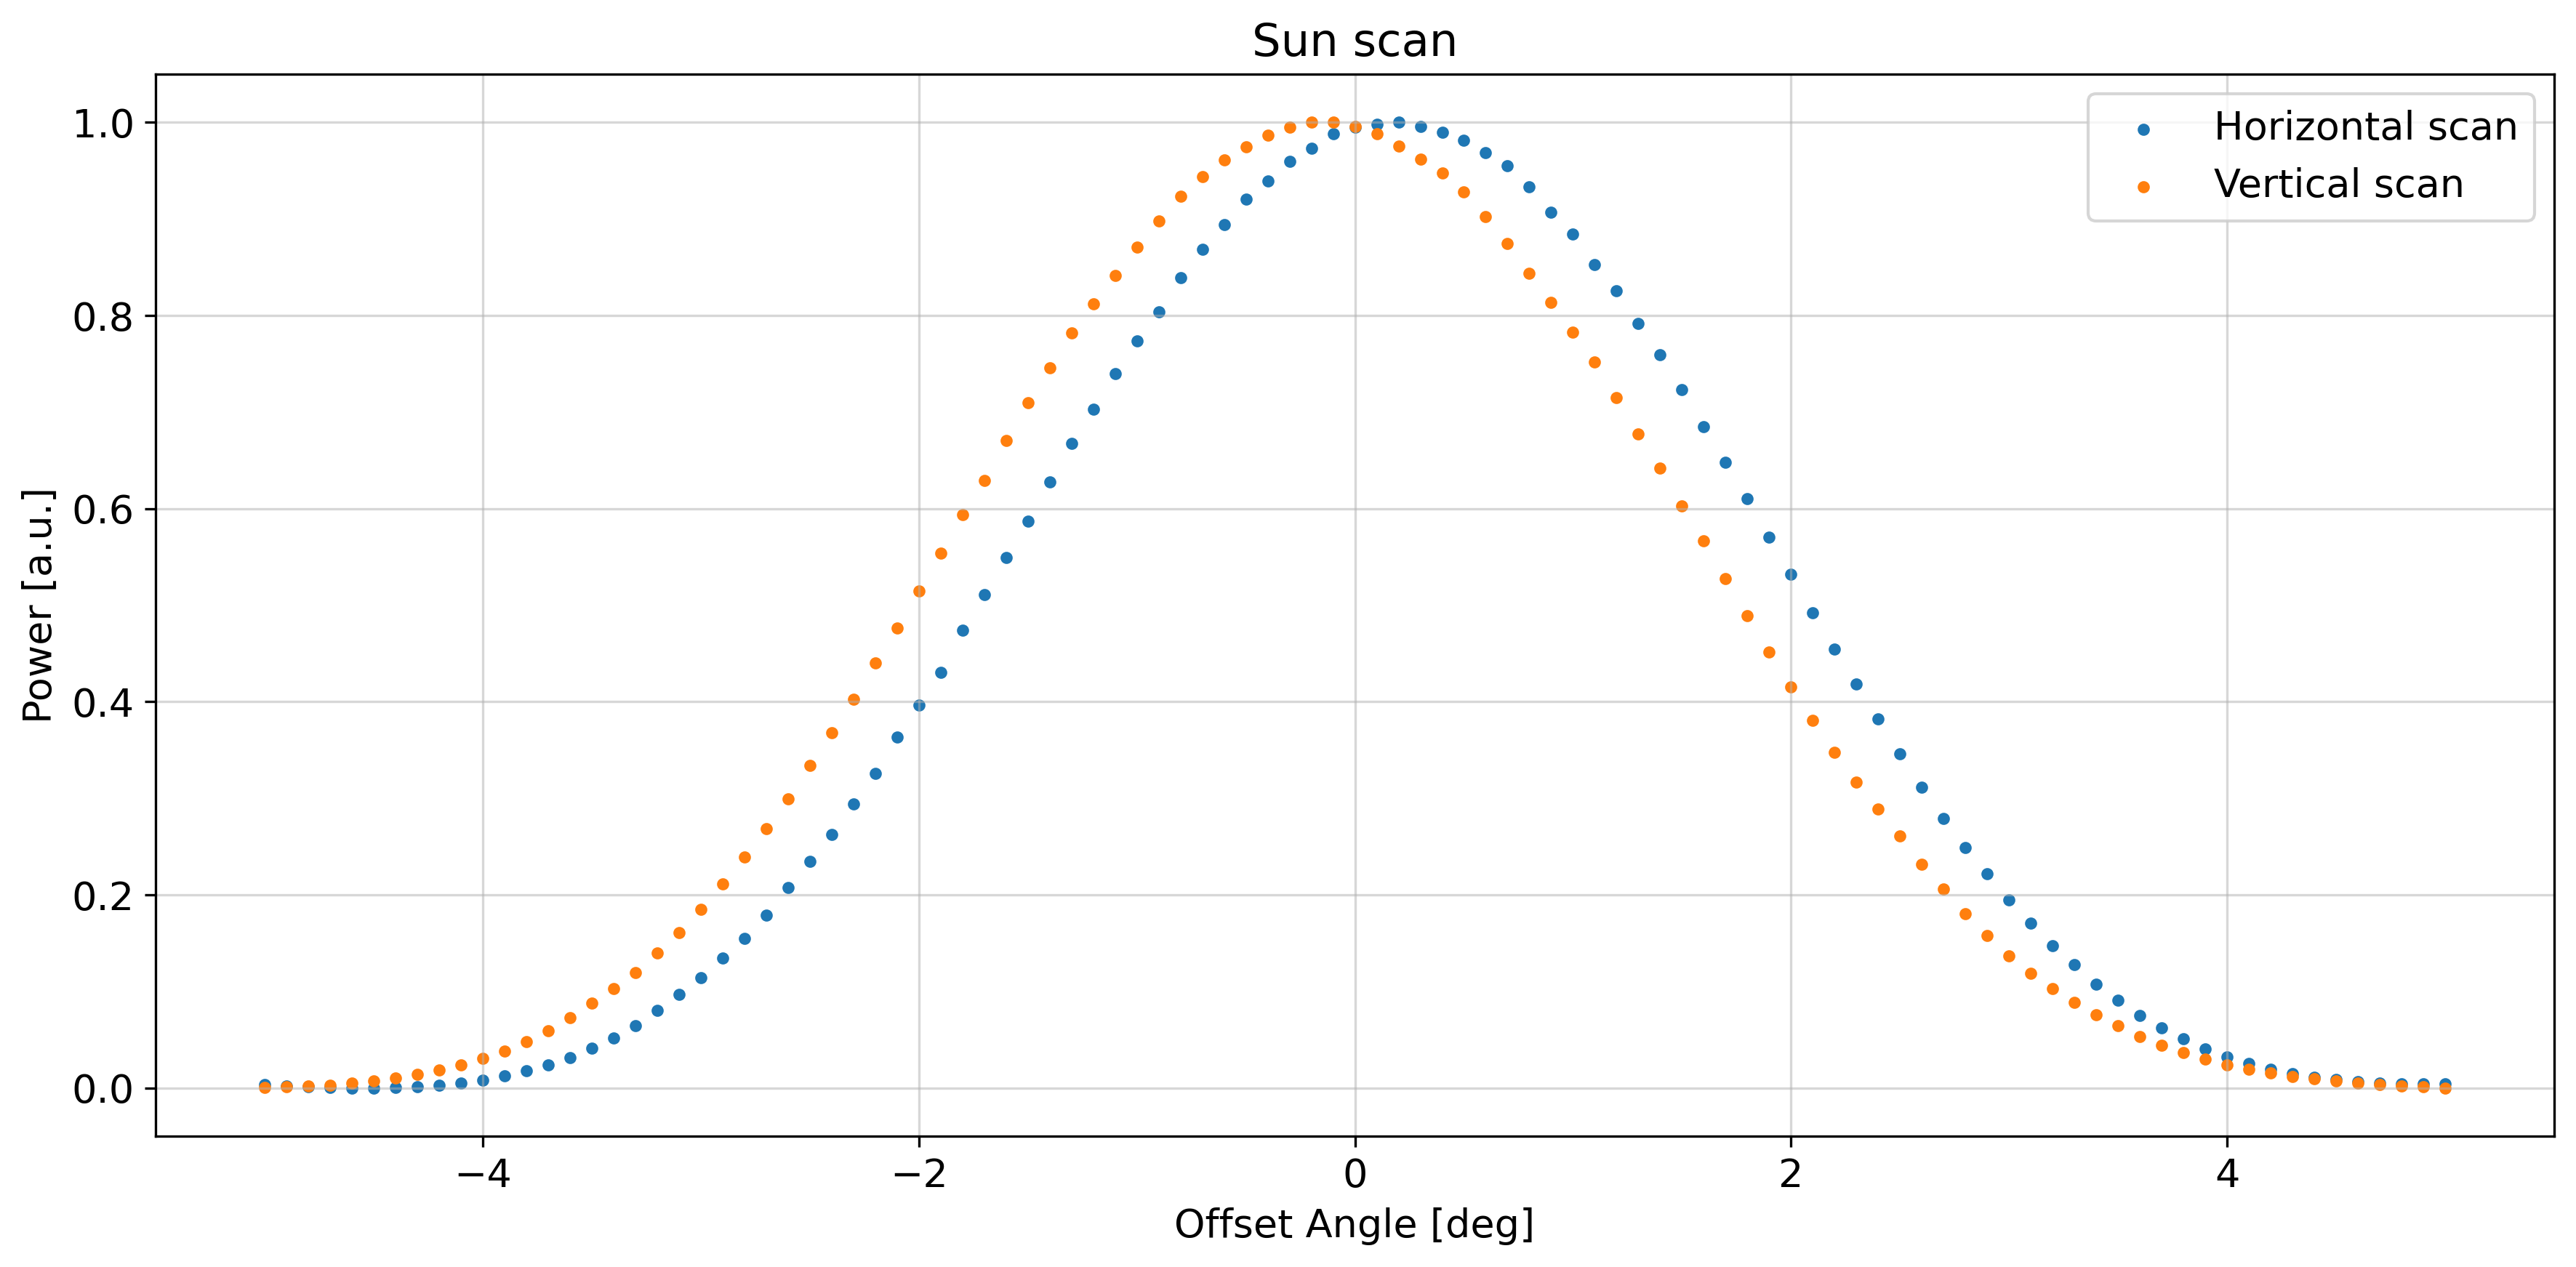
\includegraphics[width=\linewidth]{assets/sun_scan_high_res.png}
    \end{subfigure}
    \caption{Scan of the sun}
    \label{fig:sun_scan}
\end{figure}

The side bulbs are more visible when the normalizes power is shown logarithmically, this is shown in figure \ref{fig:sun_scan_log}
\begin{figure}[ht]
    \centering
    \begin{subfigure}[t]{0.45\linewidth}
        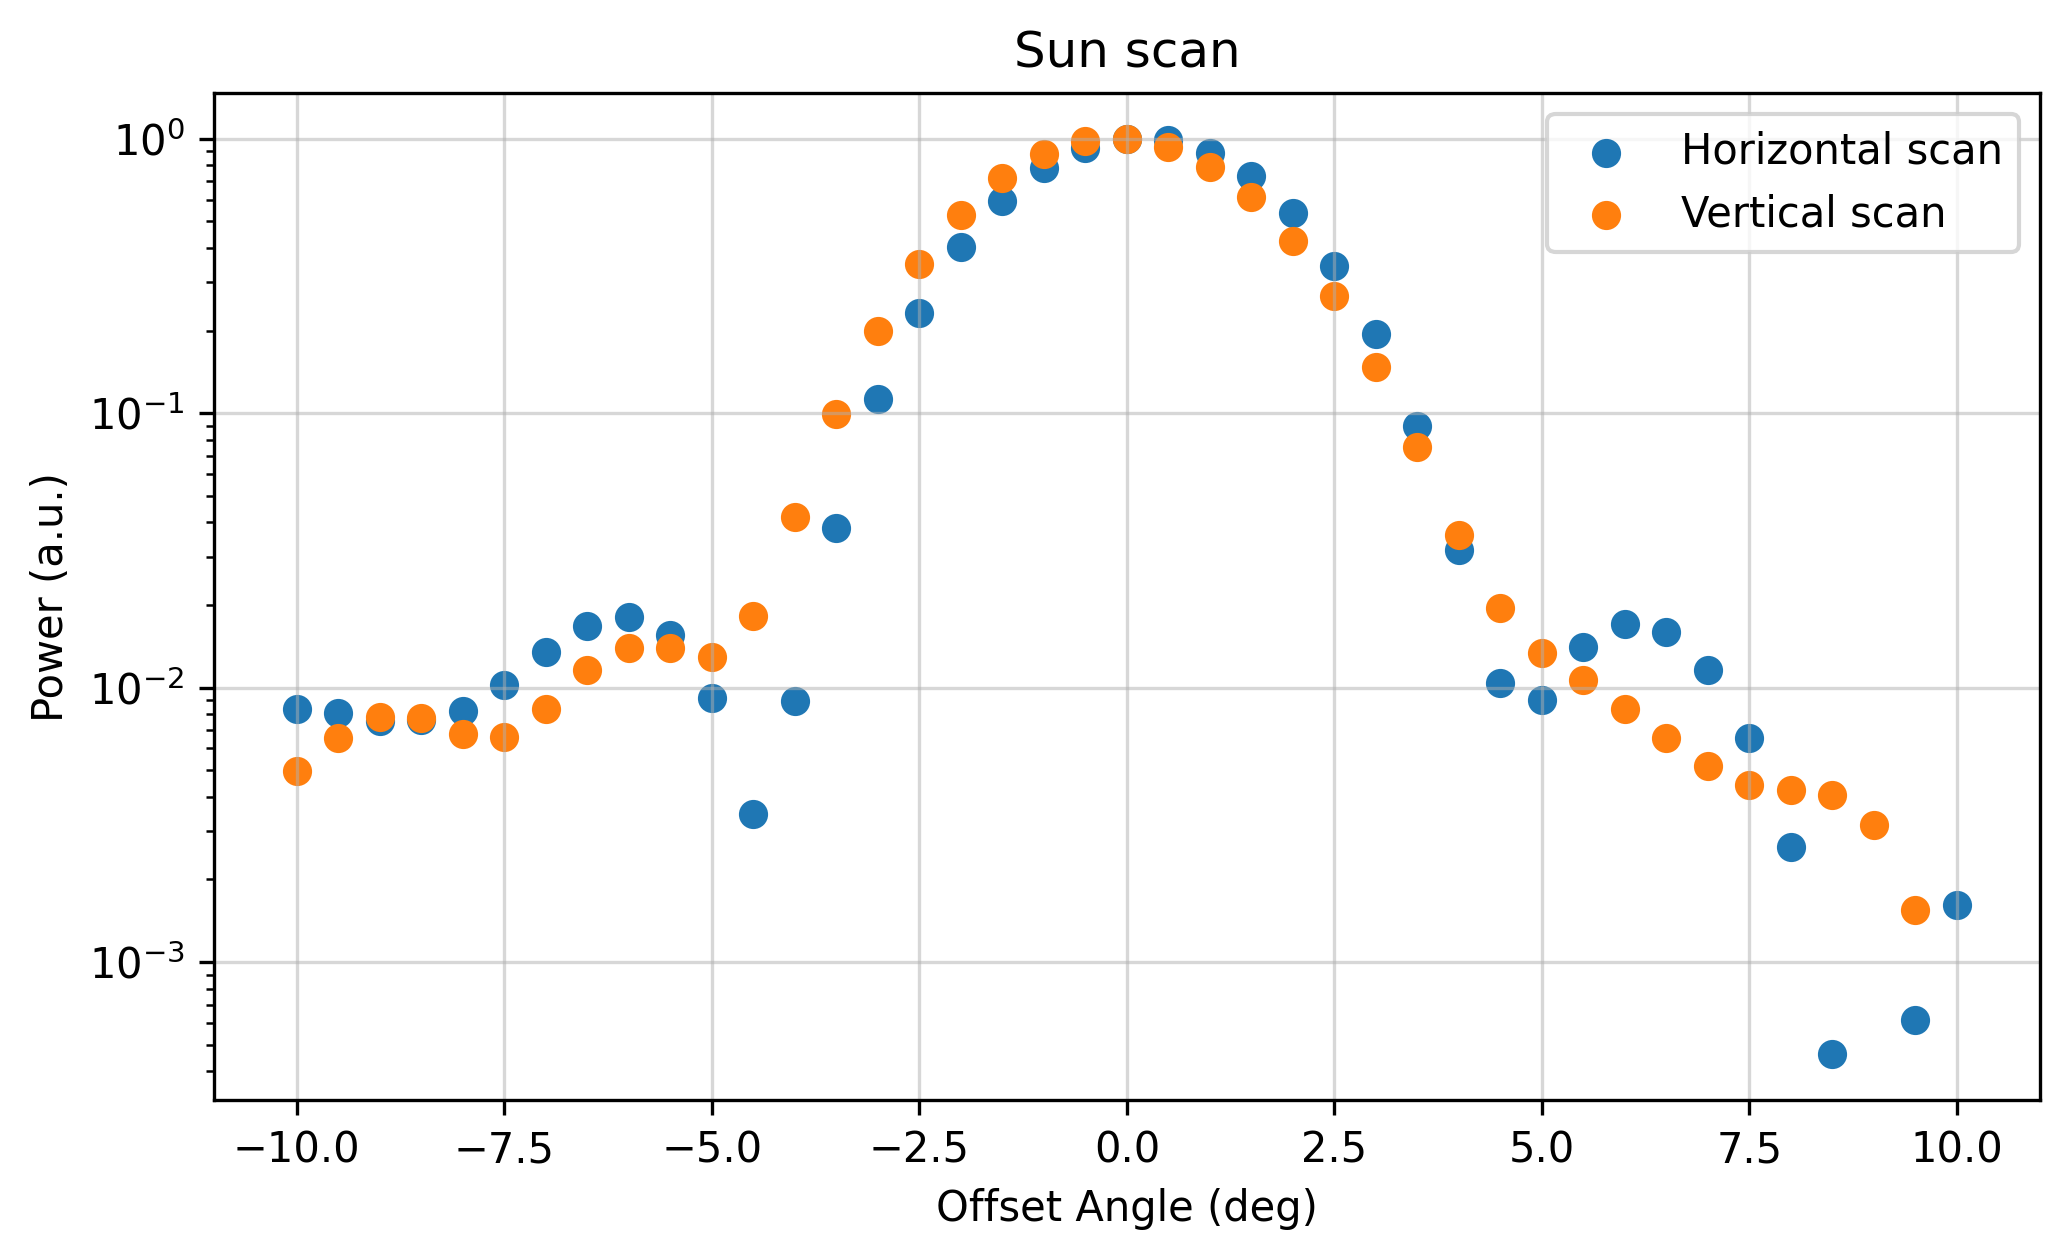
\includegraphics[width=\linewidth]{assets/sun_scan_low_res_log.png}
    \end{subfigure}
    \begin{subfigure}[t]{0.45\linewidth}
        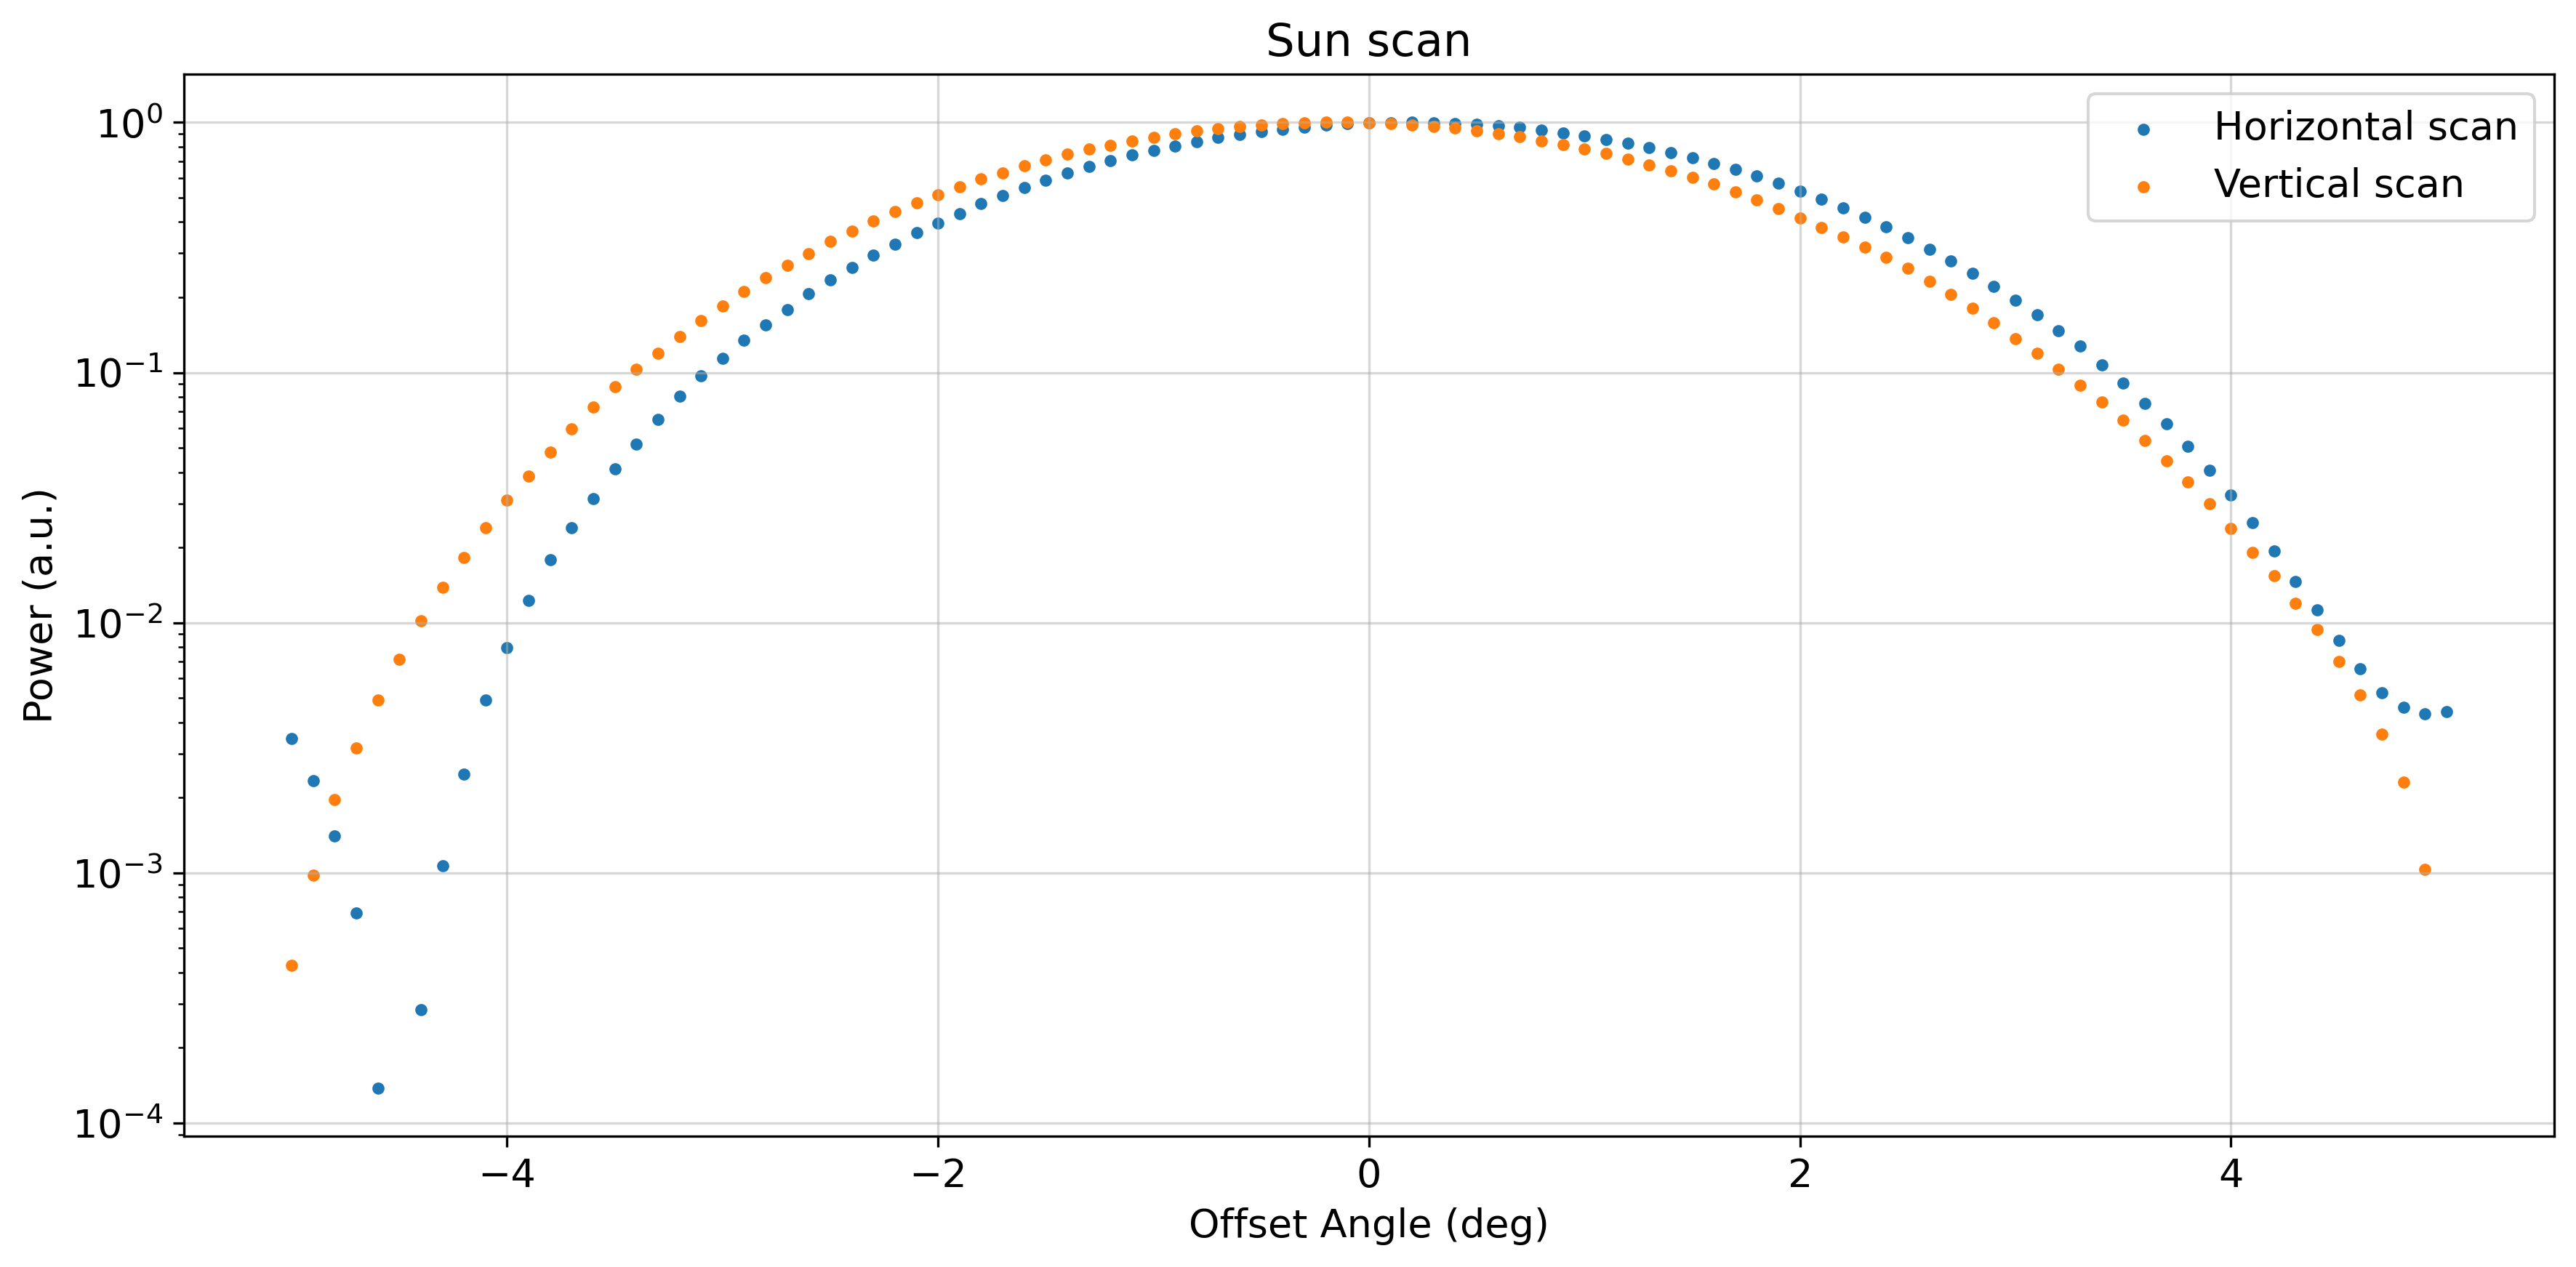
\includegraphics[width=\linewidth]{assets/sun_scan_high_res_log.png}
    \end{subfigure}
    \caption{Scan of the sun with logarithmic scale}
    \label{fig:sun_scan_log}
\end{figure}

To determine the full width at half maximum (FWHM) we use the high resolution data and fit it to a gaussian this is illustrated in figure \ref{fig:sun_scan_fit}

\begin{figure}[ht]
    \centering
    \begin{subfigure}[b]{0.45\textwidth}
        \centering
        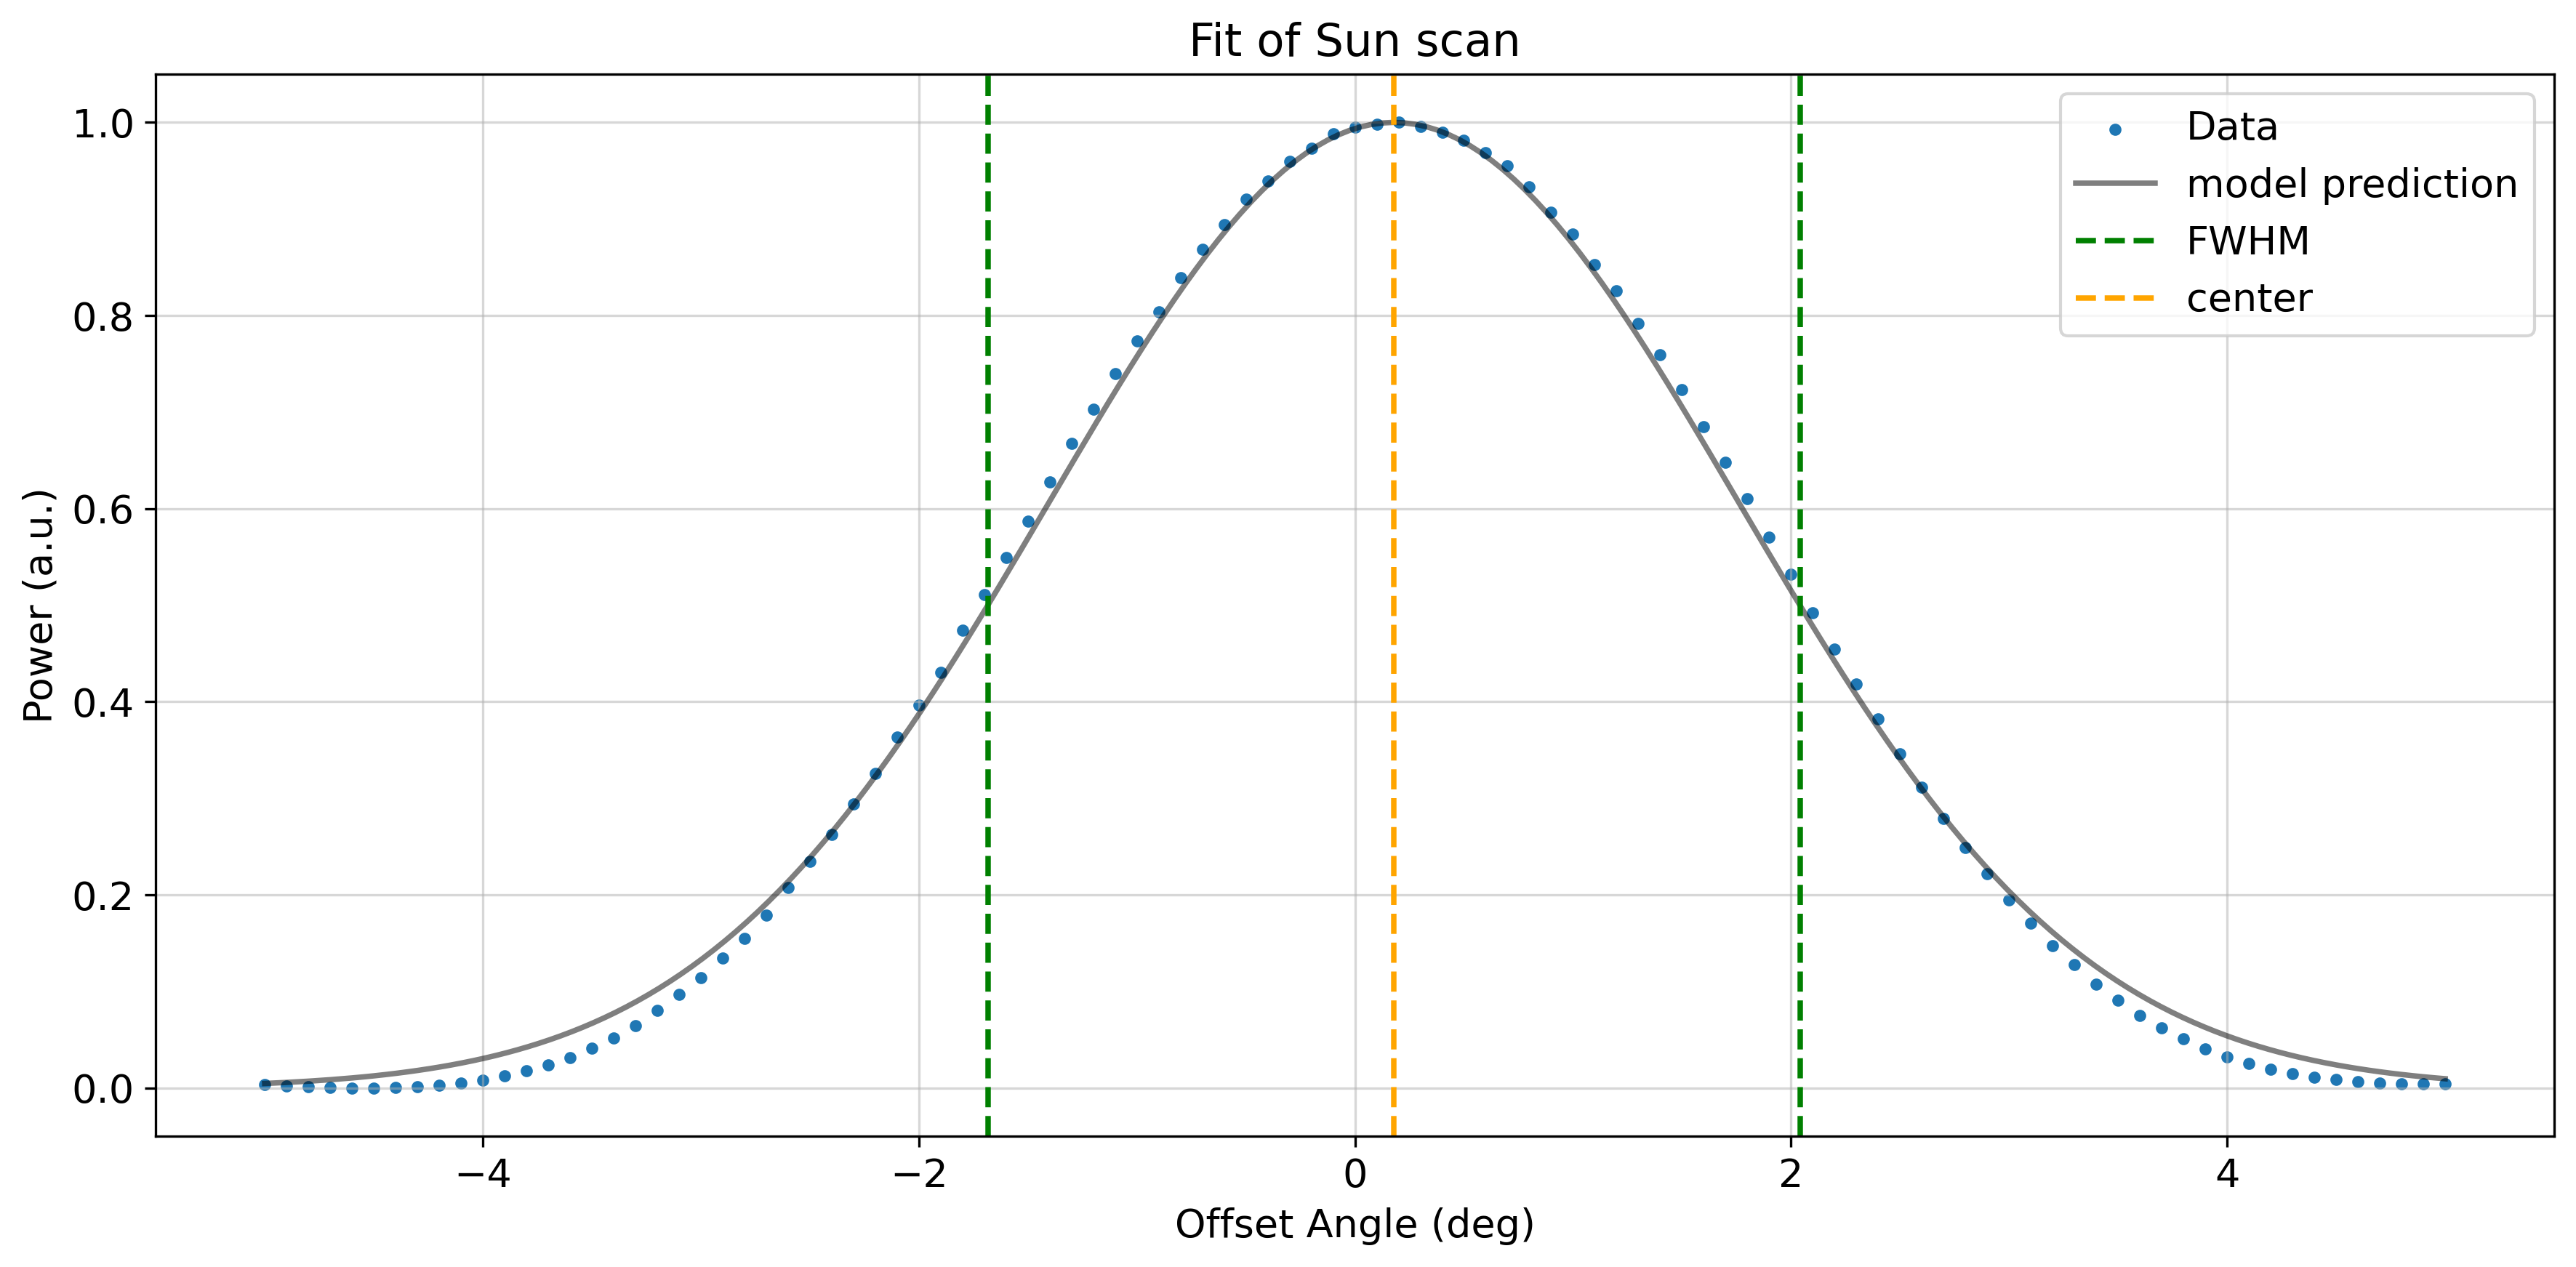
\includegraphics[width=\textwidth]{assets/sun_scan_fit_h.png}
        \caption{Horizontal fit to the data}
        \label{fig:sun_fit_h}
    \end{subfigure}
    \hfill
    \begin{subfigure}[b]{0.45\textwidth}
        \centering
        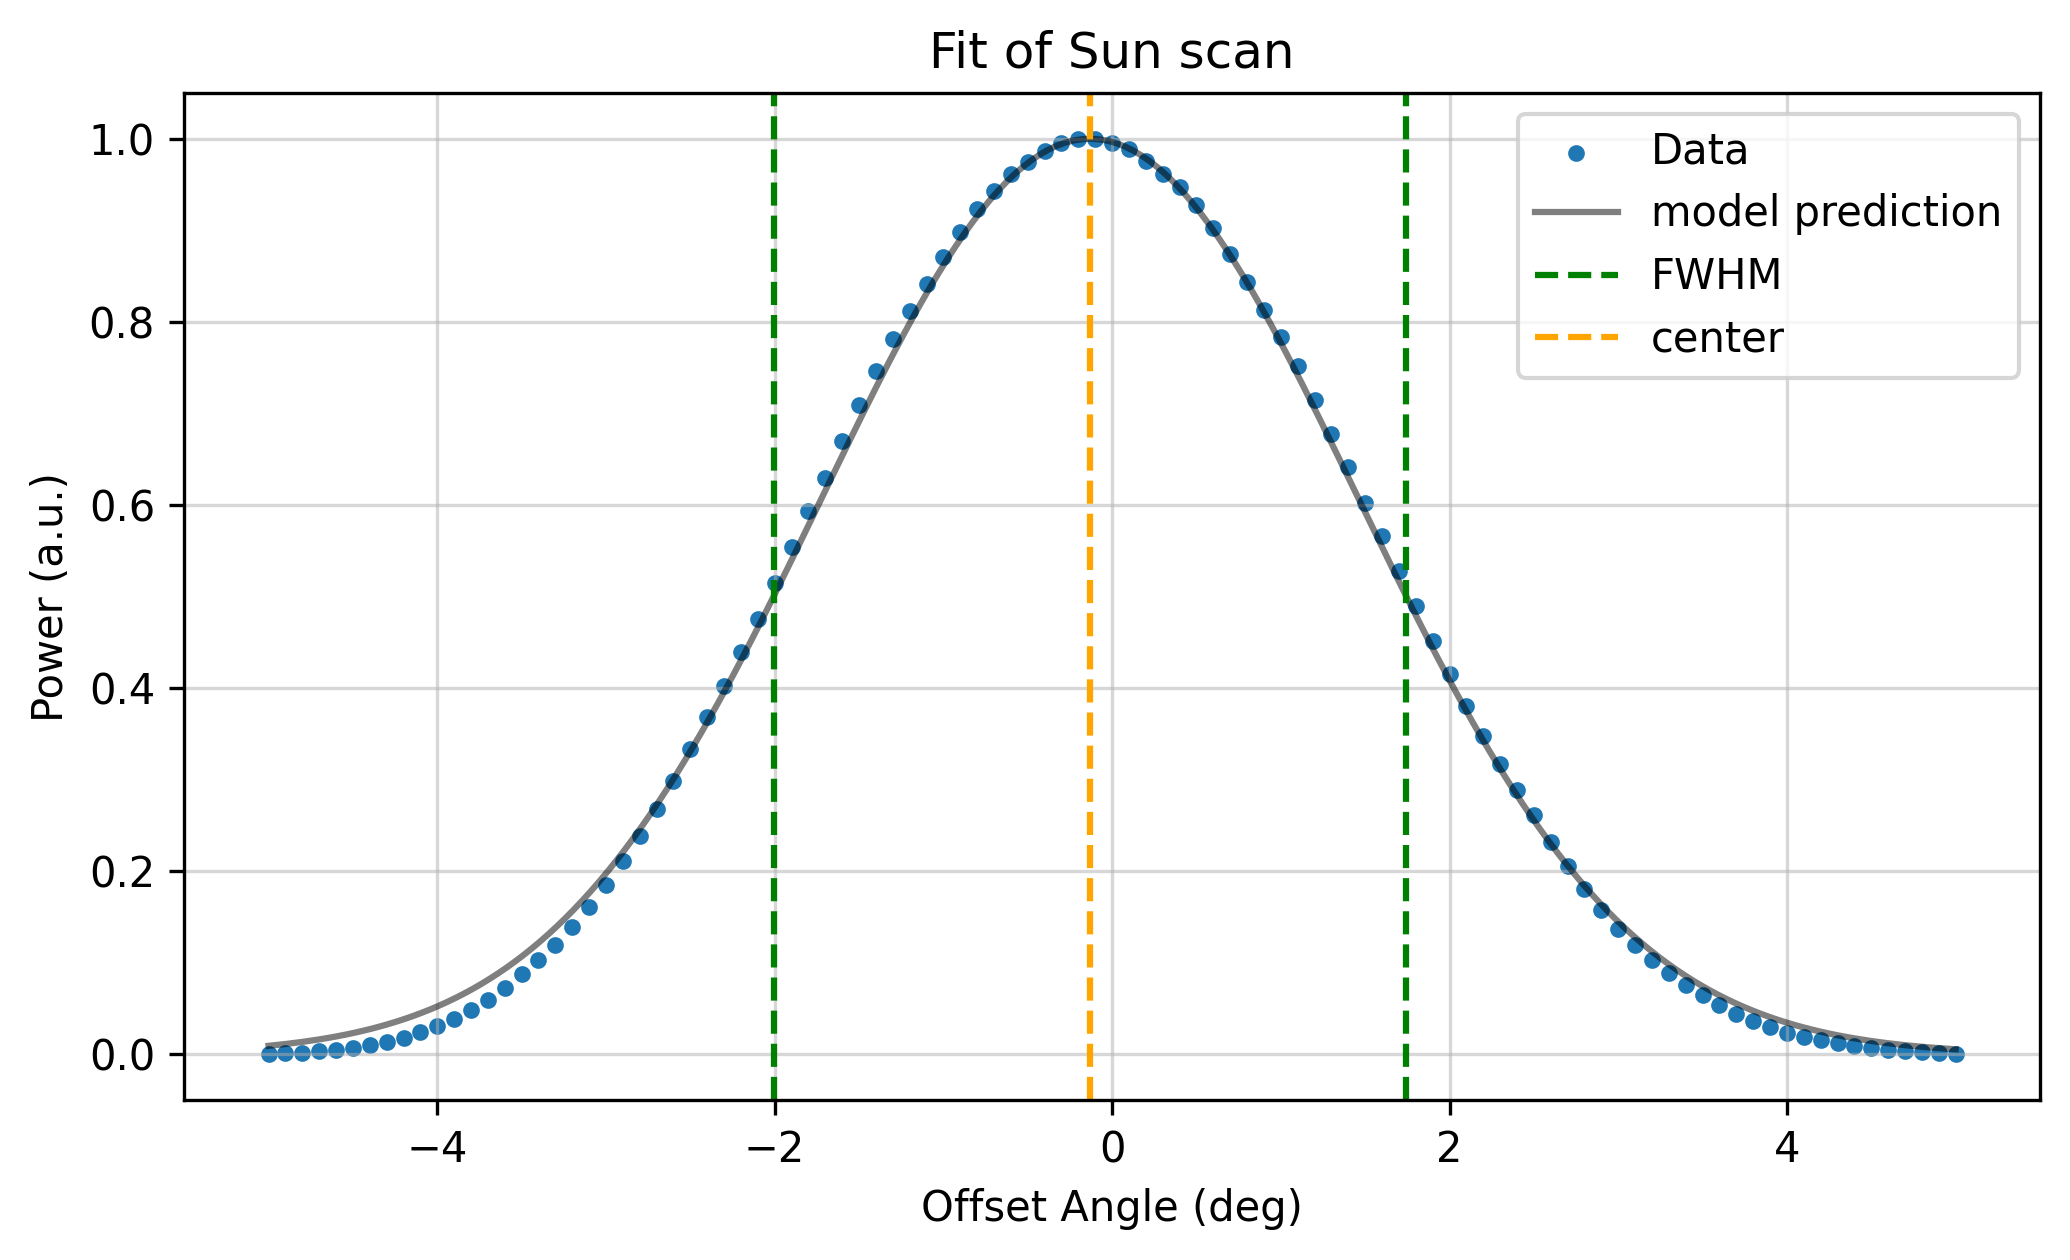
\includegraphics[width=\textwidth]{assets/sun_scan_fit_v.png}
        \caption{Vertical}
        \label{fig:sun_fit_v}
    \end{subfigure}
    \caption{;alkdsf}
    \label{fig:sun_scan_fit}
\end{figure}